\pdfoutput=1
\pdfminorversion=4

\newif\ifmeasure
%\measuretrue

\ifmeasure
\documentclass[final,twocolumn]{elsarticle}
\else
\documentclass[preprint]{elsarticle}
\fi

\usepackage[utf8]{inputenc}

%packages
\usepackage[margin=1in]{geometry}

\usepackage[hyphens]{url}
\biboptions{sort&compress, square, comma}
\usepackage[breaklinks=true, linkcolor=blue, citecolor=blue, colorlinks=true]{hyperref}

\usepackage{graphicx}
\usepackage{caption}
\usepackage{subcaption}

\captionsetup[algorithm]{labelformat=empty}

\usepackage{booktabs}
\usepackage[version=3]{mhchem} % Formula subscripts using \ce{}, e.g., \ce{H2SO4}
\usepackage{latexsym,amsmath,amssymb}

\usepackage{mathtools}
\usepackage{tablefootnote}

%better printing of numbers
\usepackage[T1]{fontenc}
\usepackage[english]{babel}
\usepackage{csquotes}
\usepackage{textcomp}

\usepackage{algorithm}
\usepackage[noend]{algpseudocode}
\makeatletter
\let\OldStatex\Statex
\renewcommand{\Statex}[1][3]{%
  \setlength\@tempdima{\algorithmicindent}%
  \OldStatex\hskip\dimexpr#1\@tempdima\relax}

\usepackage[binary-units]{siunitx}
\sisetup{group-separator={,},
     detect-all,
     binary-units,
     list-units = single,
     range-units = single,
     range-phrase = --, 
     per-mode = symbol-or-fraction,
     separate-uncertainty = true,
     multi-part-units = single,
     list-final-separator = {, and }
%    scientific-notation = fixed
}
\DeclareSIUnit\atm{atm}

% Add [disable] option to quickly remove any
\usepackage[textsize=small,textwidth=2.25cm]{todonotes}

%custom commands
\newcommand{\NA}{---}
\newcommand{\centercell}[1]{\multicolumn{1}{c}{#1}}
\newcommand{\centermulti}[2]{\multicolumn{#2}{c}{#1}}
\newcommand{\head}[1]{\centercell{\bfseries#1}}
\newcommand{\headmulti}[2]{\centermulti{\bfseries#1}{#2}}

\newcommand{\argmax}{\operatornamewithlimits{argmax}}

\journal{36th International Symposium on Combustion}

\begin{document}
\begin{titlepage}
\parbox{\linewidth}{
\begin{flushleft}
\textbf{Title:}\linebreak
An investigation of GPU-based stiff chemical kinetics integration methods
\linebreak
\linebreak
\textbf{Authors and Affiliations:} \linebreak\linebreak
  N.  Curtis	(860) 803-4660 \linebreak
  C.J Sung	(860) 486-3679 \linebreak
  Department of Mechanical Engineering \linebreak
  The University of Connecticut \linebreak
  191 Auditorium Road, Unit 3139 \linebreak
  Storrs, CT 06269-3139 \linebreak
  \linebreak
  K.E. Niemeyer	(541) 737-5614 \linebreak
  School of Mechanical, Industrial, and Manufacturing Engineering\linebreak
  Oregon State University\linebreak
\linebreak
\textbf{Corresponding Author:}\linebreak
  N. Curtis\linebreak
  (860) 803-4660 \linebreak
  Department of Mechanical Engineering\linebreak
  The University of Connecticut \linebreak
  191 Auditorium Road, Unit 3139 \linebreak
  Storrs, CT 06269-3139 \linebreak
  \href{mailto:nicholas.curtis@uconn.edu}{nicholas.curtis@uconn.edu}\linebreak
\linebreak
\textbf{Colloquium:}\linebreak
REACTION KINETICS\linebreak
\linebreak
\textbf{Word Count:}\linebreak
Method 2\linebreak
Formatted into two columns using elsarticle\linebreak
With font sizes and spacing as specified in the Latex Author Instructions.\linebreak
Six full pages $\times$ 900 words/page + 135 mm column $\times$ 2.2 words/mm = 5697 words.\linebreak
\textbf{Color Charges:}\linebreak
We do not authorize the reproduction of color images in print.
\end{flushleft}
}
\end{titlepage}

\ifmeasure
\small
\baselineskip 10pt
\fi
\begin{frontmatter}

\title{An investigation of GPU-based stiff chemical kinetics integration methods}

\author[uconn]{Nicholas~J.\ Curtis\corref{cor1}}
\ead{nicholas.curtis@uconn.edu}
\author[osu]{Kyle~E.\ Niemeyer}
\author[uconn]{Chih-Jen Sung}
%\ead{cjsung@engr.uconn.edu}

% addresses
\address[uconn]{Department of Mechanical Engineering\\
  University of Connecticut, Storrs, CT, 06269, USA}
\address[osu]{School of Mechanical, Industrial, and Manufacturing Engineering\\
  Oregon State University, Corvallis, OR 97331, USA}
  
\cortext[cor1]{Corresponding author}

\begin{abstract}
A fifth-order implicit Runge--Kutta method and two fourth-order exponential integration methods equipped with Krylov subspace approximations were implemented for the GPU and paired with the analytical chemical kinetic Jacobian code \texttt{pyJac}.
The performance of each was evaluated by integrating thermochemical state data sampled from stochastic partially stirred reactor simulations and compared with the commonly used CPU-based implicit integrator \texttt{CVODE}.
The implicit Runge--Kutta method performed over five times faster on a single GPU than \texttt{CVODE} on a single six-core CPU for an \ce{H2}\slash\ce{CO} model, and up to \SI{31.5}{\percent} faster than \texttt{CVODE} for the GRI-Mech 3.0 model.
The exponential integration techniques performed less efficiently for all cases.
The main limiter of GPU integrator performance was identified as thread divergence, and techniques to mitigate this issue were discussed.
A novel shared memory caching strategy for the GPU was developed and shown to provide a \SIrange{5}{24}{\percent} performance increase to all GPU-based integrators.
Additionally, an issue affecting storage of the chemical kinetic Jacobian in per-thread local memory was identified and work-around methods were discussed.
Finally, future research directions were identified based on the current state-of-the-art of stiff chemical kinetics integration on the GPU.
\end{abstract}

\begin{keyword}
 Chemical kinetics \sep Stiff chemistry \sep Integration algorithms \sep GPU
\end{keyword}

\end{frontmatter}

\clearpage

%%%%%%%%%%%%%%%%%%%%%%%%%%%%%%%%%%%%%%%%%%%%
\section{Introduction}
\label{sec:Intro}
\ifmeasure
\addvspace{10pt}
\fi
%%%%%%%%%%%%%%%%%%%%%%%%%%%%%%%%%%%%%%%%%%%%

The need for accurate chemical kinetic models in predictive reacting-flow simulations has driven the development of detailed oxidation models for hydrocarbon fuels relevant to transportation and energy generation applications.
At the same time, growing understanding of hydrocarbon oxidation processes resulted in orders of magnitude increases in model size and complexity.
For instance, a recently developed model for 2-methylalkanes, relevant for jet and diesel fuel surrogates, includes over 7000 species and 30000 reactions~\cite{Sarathy:2011kx} while a recent detailed gasoline surrogate mechanism contains over 1500 species and 6000 reactions~\cite{Mehl:2011jn}.
Furthermore, kinetic models for large hydrocarbon fuels tend to exhibit high chemical stiffness that requires implicit integration algorithms for efficient solution.
The cost of these algorithms scales at best quadratically---and at worst cubically---with the number of species in a model~\cite{Lu:2009gh}.
Lu and Law~\cite{Lu:2009gh} extensively reviewed techniques to accelerate chemical kinetics integration.
In addition to the methods discussed in their work, significant effort has also been directed towards improvements of the integration algorithms.

Reactive-flow modeling codes commonly rely on high-order implicit integration techniques to solve the stiff governing equations posed by chemical kinetic models.
These methods require repeated evaluation and factorization of the chemical kinetic Jacobian matrix in order to solve the associated nonlinear algebraic equations through iterations of linear system solutions---the cost of which scales quadratically and cubically, respectively, with the number of species in a mechanism.
However, significant cost savings in the Jacobian evaluation can be realized by using an analytical formulation, rather than the typical evaluation via finite difference approximations.
This approach eliminates numerous chemical source term evaluations, and for a sparse Jacobian (e.g., formulated in terms of species concentrations) the cost of evaluation drops to a linear dependence on the number of species in the mechanism~\cite{Lu:2009gh}.

In this study, our efforts to accelerate chemical kinetics focus on improving the integration strategy itself, via development of new algorithms and use of high-performance hardware accelerators such as graphics processing units (GPUs) and other similar single instruction multiple data (SIMD) devices.
Central processing unit (CPU) clock speeds increased regularly over the past few decades---commonly known as Moore's Law---however, power consumption and heat dissipation issues slowed this trend recently.
While multicore parallelism somewhat increased CPU performance, recently SIMD processors gained popularity as a low cost, low power consumption, and massively parallel high-performance computing alternative.
GPUs were originally developed for graphics\slash video processing applications and consist of hundreds to thousands of separate cores, compared with the tens of cores found on typical CPUs.
The SIMD parallelism model differs from a traditional CPU-based multithreading model, with small per-core memory caches and acceleration resulting from executing the same instruction over multiple data.
For more details, we refer the reader to several works that discussed these differences in depth~\cite{Cruz:2011gc,Brodtkorb:2013hn,Niemeyer:2014hn}.

A number of studies in recent years explored the use high-performance SIMD devices to accelerate (turbulent) reacting-flow simulations.
Spafford et al.~\cite{Spafford:2010aa} investigated using GPUs to accelerate a turbulent combustion direct numerical simulation code, demonstrating a sub-order of magnitude speedup in evaluating the species production rates on the GPU.
Shi et al.~\cite{Shi:2011aa} used a GPU to evaluate species rates and factorize the Jacobian for the integration of independent kinetics systems, showing order-of-magnitude or greater speedups for large kinetic models.
Niemeyer et al.~\cite{Niemeyer:2011aa} implemented an explicit fourth-order Runge--Kutta integrator for the GPU, and found a speedup of nearly two orders of magnitude with a nonstiff hydrogen mechanism.
Shi et al.~\cite{Shi:2012aa} implemented a stabilized explicit solver for the GPU and paired it with a CPU-based implicit solver that handled integration of the most-stiff chemistry cells in a three-dimensional premixed diesel engine simulation, demonstrating an overall speedup of \numrange{2}{3}$\times$.
Le et al.~\cite{Le2013596} implemented GPU versions of two high-order shock-capturing reacting flow codes, and found a \numrange{30}{50}$\times$ speedup over the baseline.
Stone and Davis~\cite{Stone:2013aa} implemented the implicit VODE~\cite{Brown:1989vl} solver for the GPU and achieved an order of magnitude speed-up over the baseline CPU version.
Additionally, they showed that the implicit VODE algorithm exhibited significant thread divergence, as expected due to its complicated program flow (compared with an explicit integration scheme).
Furthermore, Stone and Davis~\cite{Stone:2013aa} showed that, for numbers of independent ODE systems greater than $\sim$\SI{e3}, using individual GPU threads to handle independent chemical kinetic ODEs offered greater performance over using a block of GPU threads to cooperatively solve a single ODE.
Niemeyer and Sung~\cite{Niemeyer:2014aa} demonstrated an order-of-magnitude speedup for a GPU implementation of a stabilized explicit second-order Runge--Kutta--Chebyshev algorithm over a multicore CPU implementation of VODE for moderately stiff chemical kinetics.
They also investigated levels of thread divergence due to differing integrator time-step sizes, and found it negatively impacts overall performance for dissimilar ODE initial conditions in a thread-block.
Sewerin and Rigopoulos~\cite{Sewerin20151375} implemented a three-stage\slash fifth-order implicit Runge--Kutta method~\cite{wanner1991solving} on a one-block per ODE basis on GPU, and found a \num{1.8}$\times$ slowdown at best compared with the same on a single eight-core CPU.

While increasing numbers of studies have explored GPU-based chemical kinetics integration, there remains a clear need to find or develop integration algorithms simultaneously suited for the SIMD parallelism of GPUs (along with similar hardware accelerators) and capable of handling stiffness.
In this work we will investigate GPU implementations of several explicit and implicit integration techniques, as compared to their CPU counterparts and the baseline CPU \texttt{CVODE}~\cite{Hindmarsh:2005hg} algorithm.
Several previous works~\cite{Perini20141180,McNenly2015581} suggested so-called matrix-free methods---which do not require direct factorization of the Jacobian, but instead use an iterative process to approximate the action of the factorized Jacobian on a vector---as potential improvements to the expensive linear-system solver required in standard implicit methods.
Furthermore, Hochbruck and Lubich~\cite{Hochbruck:1997} demonstrated that the action of the matrix exponential on a vector obtained using Krylov subspace approximation converges faster than corresponding Krylov methods for the solution of linear equations.
Others previously explored these so-called explicit exponential methods for applications in stiff chemical systems~\cite{Bisetti:2012jw,falati2011integration} and found them stable for time-step sizes greatly exceeding the stability bound.
In addition, their explicit nature makes them potentially much better suited for SIMD acceleration due to an expected reduction of thread divergence compared with implicit methods.
Finally, the three-stage fifth-order implicit Runge--Kutta algorithm~\cite{wanner1991solving} investigated by Sewerin and Rigopoulos~\cite{Sewerin20151375} will be studied to determine the impact of increasing chemical stiffness on the algorithm and the performance benefits of using an analytical Jacobian matrix, such as that developed by Niemeyer et al.~\cite{Niemeyer:2015im,Niemeyer:2015ws}.

%%%%%%%%%%%%%%%%%%%%%%%%%%%%%%%%%%%%%%%%%%%%
\section{Methodology}
\label{sec:Method}
\ifmeasure
\addvspace{10pt}
\fi
%%%%%%%%%%%%%%%%%%%%%%%%%%%%%%%%%%%%%%%%%%%%

In this section, we discuss details of the algorithms implemented for the GPU along with third-party software used.
The generation of testing conditions will be discussed briefly, and a shared memory caching algorithm will be outlined.

%%%%%%%%%%%%%%%%%%%%%%%%%%%%%%%%%%%%%%%%%%%%
\subsection{Integration techniques}

We investigated GPU implementations of three integration methods in this work, comparing them against equivalent CPU versions and a CPU-only implicit algorithm.
While we describe important details or changes here, full descriptions of all algorithms may be found in the cited sources.
The \texttt{pyJac} software~\cite{Niemeyer:2015im,Niemeyer:2015ws} provided both chemical source term and analytical Jacobian subroutines for CPU- and GPU-based algorithms.
For validation and performance assessments of \texttt{pyJac}, we direct readers to our previous work~\cite{Niemeyer:2015ws}.

First, we used the \texttt{CVODE} solver~\cite{Hindmarsh:2005hg} to provide the baseline performance of a typical CPU-based (maximum of fifth-order) implicit integration technique.
In addition, we implemented CPU versions of the methods under investigation for direct comparison to the high-order implicit technique.
These include the three-stage/fifth-order implicit Runge--Kutta algorithm~\cite{wanner1991solving}, called \texttt{Radau-IIA} here; the fourth-order exponential Rosenbrock-like method \texttt{exp4} of Hochbruck et al.~\cite{Hochbruck:1998}; and the newer fourth-order exponential Rosenbrock method~\cite{Hockbruck:2009}, called \texttt{exprb43} here.
For the exponential methods, we used the method of rational approximants~\cite{gallopoulos:1992} paired with the Carath\'edothy--Fej\'er method~\cite{trefethen:2006} to approximate the action of the matrix exponential on a vector, as suggested by Bisetti~\cite{Bisetti:2012jw}.
This technique relied on the external \texttt{FFTW3} library~\cite{frigo2005design}.
However, unlike the approach of Bisetti~\cite{Bisetti:2012jw}, we developed a custom routine based on the algorithm presented by Stewart~\cite{stewart:1998} to perform LU decomposition of the Hessenberg matrix resulting from the Arnoldi iteration.
To ensure high performance of CPU-based methods, the Intel \texttt{MKL} library version 11.1.3 handled linear algebra (i.e., BLAS/LAPACK) operations.
Next, we implemented GPU versions of the \texttt{Radau-IIA}, \texttt{exp4}, and \texttt{exprb43} methods; these follow the same descriptions as the CPU versions, but required specialized implementations of several BLAS and LAPACK methods, mostly related to LU factorization of the Jacobian or Hessenberg matrices.
All GPU routines were developed using the NVIDIA CUDA framework~\cite{Buck:2008aa,NVIDIA:2015aa}.
Finally, the adaptive time stepping procedures of all integrators used absolute and relative tolerances of \SI{e-15} and \SI{e-8}, respectively, throughout the work, and the exponential integrators used a rational approximant type of $\left(10,10\right)$ as suggested by Bisetti~\cite{Bisetti:2012jw}.

%%%%%%%%%%%%%%%%%%%%%%%%%%%%%%%%%%%%%%%%%%%%
\subsection{Testing conditions}
\label{S:pasr_conditions}

In order to measure the performance of the integrators for realistic conditions, a database of thermochemical states covering a wide range of temperatures and species mass fractions was generated using a previously developed constant-pressure stochastic partially stirred reactor (PaSR) code~\cite{Niemeyer:2015ws}.
We selected two chemical kinetic models to span the range of model sizes typically used in high-fidelity simulations: the \ce{H2}\slash\ce{CO} model of Burke et al.~\cite{Burke:2011fh} with 13 species and 27 reactions, and the GRI-Mech 3.0 model with 53 species and 325 reactions~\cite{smith_gri-mech_30}.
The PaSR simulations were performed at the conditions listed in Table~\ref{T:pasr_parameters} for 10 residence times to reach a statistical steady state; Niemeyer et al.~\cite{Niemeyer:2015ws} described the PaSR simulation process in greater detail, which follows approaches used by others~\cite{Chen:1997ta,Pope:1997wu,Ren:2014cd}.
%
%\label{S:pasr}
%\begin{table}[htb]
%\centering
%\fontsize{8pt}{10pt}\selectfont
%\begin{tabular}{@{}l l l l@{}}
%\toprule
%Fuel species & \# of species & \# of reactions & Reference \\
%\midrule
%\ce{H2}\slash \ce{CO} & 13 & 27 &~\cite{Burke:2011fh} \\
%\ce{CH4} & 53 & 325 &~\cite{smith_gri-mech_30} \\
%\bottomrule
%\end{tabular}
%\caption{
%Summary of chemical kinetic models used as benchmark test cases.
%}
%\label{T:mechanisms}
%\end{table}

\begin{table}[htb]
\centering
\ifmeasure
\fontsize{8pt}{10pt}\selectfont
\fi
\begin{tabular}{@{}l l l @{}}
\toprule
Parameter & \ce{H2}\slash air & \ce{CH4}\slash air \\
\midrule
$\phi$ & \multicolumn{2}{c}{1} \\
$T_{\text{in}}$ & \multicolumn{2}{c}{\SIlist{400;600;800}{\kelvin}} \\
$p_0$ & \multicolumn{2}{c}{\SIlist{1;10;25}{\atm}} \\
$N_p$ & \multicolumn{2}{c}{100} \\
$\tau_{\text{res}}$ & \SI{10}{\milli\second} & \SI{5}{\milli\second} \\
$\tau_{\text{mix}}$ & \SI{1}{\milli\second} & \SI{1}{\milli\second} \\
$\tau_{\text{pair}}$ & \SI{1}{\milli\second} & \SI{1}{\milli\second} \\
\bottomrule
\end{tabular}
\caption{
PaSR parameters used for hydrogen\slash air and methane\slash air premixed combustion cases, where $\phi$ indicates equivalence ratio, $T_{\text{in}}$ is the temperature of the inflowing particles, $p_0$ is the pressure, $N_p$ is the number of particles, $\tau_{\text{res}}$ is the residence time, $\tau_{\text{mix}}$ is the mixing time, and $\tau_{\text{pair}}$ is the pairing time.
}
\label{T:pasr_parameters}
\end{table}

%%%%%%%%%%%%%%%%%%%%%%%%%%%%%%%%%%%%%%%%%%%%
\subsection{Shared memory caching}
\label{S:smem_present}

A unique memory-access pattern is one aspect of the GPU platform particularly important to high-performance algorithms; each streaming multiprocessor can access only a small amount of fast cache memory (typically \SI{64}{\kilo\byte}) and \SI{32}{\bit} registers (typically \SIrange{32}{64}{\kilo\byte}).
All other memory is stored globally on the device, with comparatively high latencies.
Thus, it is critical to properly use cache memory to achieve maximum performance on GPUs.
When formulated on a per-block basis, GPU-based integration algorithms typically use this memory to store commonly used values such as the current state vector and  chemical Jacobian.
However, on a per-thread basis, the best use of this memory is less clear; this section proposes one approach for efficient use of this fast memory.

Using fast memory on a per-thread basis poses a challenge: it must be split between all threads in the blocks resident on a streaming multiprocessor.
This fast memory is further split into an L1 cache and shared memory available for interthread communication within a block.
Most versions of the CUDA compute standards allow the user to specify the relative allocation of the L1 cache and shared memory pool.
In our preliminary studies, a larger L1 cache proved the superior choice for our per-thread approach; the inherent increased memory traffic quickly overwhelms the small cache memory, resulting in slower global memory accesses.
However, this left $\sim$\SI{16}{\kilo\byte} of the cache memory as shared memory, with only around two to four double-precision variables available per thread.
This small amount of available memory is challenging to use in the integration algorithm itself; however, evaluation of the chemical source terms and analytical Jacobian present opportunities for using the shared memory.

\begin{algorithm}[htb]
\ifmeasure
\fontsize{8pt}{10pt}\selectfont
\caption{\fontsize{9pt}{10pt}\selectfont \textbf{Algorithm:} A procedure for memory caching during evaluation of reaction rates.\label{A:shared_mem_caching}}
\else
\caption{\textbf{Algorithm:} A procedure for memory caching during evaluation of reaction rates.\label{A:shared_mem_caching}}
\fi
\begin{algorithmic}[0]
  \State {Initialize the cached species concentration set $C = \varnothing$}
  \State {Let maximum set size be $C_{\max}$}
  \For {reaction $r_i$ of reactions $R$}
    \State Let $S_i$ be the set of participating species in $r_i$
    \State Let $P_{i,j}$ be the number of consecutive reactions starting from $r_{i + 1}$ in which each species $s_{i,j} \in S_i$ participates
    \State For each species $c_j \in C$ let $L_j$ be the number of reactions since $c_j$ directly participated in a reaction
    \State Priority sort the species $s_{i,j}$ in $S_{i}$ in descending order by priority $P_{i,j}$ and store in $S_{i}^{\prime}$
    \For {$s_{i,j}$ in $S_{i}^{\prime}$}
      \If{$|C| < C_{\max}$}
		\State Add $s_{i,j}$ to $C$
      \ElsIf{$\max_j \left( L_j \right) \geq 2$ and $P_{i,j}$ > 1}
	  \State Let $k = \argmax_j \left(L_j \right)$
	  \State Remove $s_{i,j}$ from $S_{i}^{\prime}$ and replace $c_k$ in $C$ with $s_{i,j}$
      \EndIf
    \EndFor
    \For {$s_{i,j}$ in $S_{i}^{\prime}$}
      \If{$| S_{i}^{\prime} | > 0$ and $ |C| < C_{\max}$}
		\State Add $s_{i,j}$ to $C$
      \EndIf
    \EndFor
    \State Compute $i$th reaction rate using values in $C$ where appropriate.
  \EndFor
\end{algorithmic}
\end{algorithm}

The presented~\hyperref[A:shared_mem_caching]{algorithm} describes a strategy to use this available shared memory to store commonly used species concentrations during evaluation of the reaction rates.
Similar algorithms were developed for the species net production rates and Jacobian evaluation routines, using frequently updated species net production rates and frequently used reaction rates\slash species concentrations as the cached variables, respectively.
As this algorithm runs during generation of the source code for the various subroutines, it introduces no computational or memory overhead related to determining the caching structure during runtime.
Although this represents a relatively simple improvement, its use can achieve reasonable performance benefits, as will be seen in Sec.~\ref{S:smem}.

%%%%%%%%%%%%%%%%%%%%%%%%%%%%%%%%%%%%%%%%%%%%
\section{Results and discussion}
\ifmeasure
\addvspace{10pt}
\fi
%%%%%%%%%%%%%%%%%%%%%%%%%%%%%%%%%%%%%%%%%%%%

We studied the performance of the integrators by testing each on the PaSR conditions described in Sec.~\ref{S:pasr_conditions} for two different global integration time-step sizes representative of those used in large eddy and Reynolds-averaged Navier--Stokes simulations: $\delta t = \SI{e-6}{\s}$ and $\delta t = \SI{e-4}{\s}$, respectively.
Furthermore, the use of a larger global time step induces additional stiffness for a given model and enables evaluation of integrator performance at varying stiffness levels.
Runtimes are reported as the average over five runs, where each run started from the same set of PaSR conditions.
While the computed runtimes exhibited some variations, we chose to omit error bars from the plots for clarity; in general, the implicit methods exhibited variations within \SI{\pm3}{\percent} and the exponential methods within \SI{\pm1}{\percent}.
All CPU integrators were compiled using \texttt{gcc 4.4.7} (with the compiler options ``\texttt{-O3 -funroll-loops -mtune=native}''), and were executed in parallel via OpenMP on a six-core \SI{2.67}{\giga\hertz} Intel Xeon X5650 with \SI{256}{\kilo\byte} of L2 cache memory per core and \SI{12}{\mega\byte} of L3 cache memory.
The same CPU served as host for the GPU integrators, which were compiled using \texttt{nvcc 7.0.27} (with compiler options ``\texttt{-arch=sm\_20 -O3 -maxrregcount 63 -{}-ftz=false -{}-prec-div=true -{}-prec-sqrt=true -{}-fmad=false}'') and run on a single NVIDIA Tesla C2075 with \SI{6}{\giga\byte} of global memory.
Reported runtimes for the GPU-based algorithms include time needed for CPU--GPU data transfer before and after each global time step; in addition, the function \texttt{cudaSetDevice()} was used to initialize the GPU before timing to hide any device initialization delay.
The open-source \texttt{pyJac} software~\cite{Niemeyer:2015im,Niemeyer:2015ws} produced CPU and GPU custom source-code functions for the chemical source terms and analytical Jacobian matrix evaluation.
In this section, the best and worst performance will be reported for cases when the GPU became fully utilized, to present unbiased performance results.
In practice, we determined this point based on when the runtime began to increase linearly with the number of ODEs---this occurred at \num{16384} ODEs for both models.
All of the GPU performance results shown in this section used the shared memory caching algorithm discussed in Sec.~\ref{S:smem_present}, the benefit of which will be discussed in Sec.~\ref{S:smem}.

\subsection{Performance}
\ifmeasure
\addvspace{10pt}
\fi

Figure~\ref{F:H2_perf} shows the runtimes of the CPU and GPU integrators for the \ce{H2}\slash\ce{CO} model.
The CPU \texttt{Radau-IIA} integrator was at best \SI{14}{\percent} faster than \texttt{CVODE} (at \num{65536} ODEs) and at worst \SI{16}{\percent} slower (at \num{32768} ODEs) for the smaller global time-step size.
In the best case for the larger global time-step size, the CPU \texttt{Radau-IIA} solver was at best \SI{3.8}{\percent} slower than \texttt{CVODE} (\num{32768} ODEs) and \SI{35}{\percent} slower at worst (\num{16384} ODEs).
For the smaller time-step size, the GPU \texttt{Radau-IIA} integrator was at best \num{5.31}$\times$ faster than \texttt{CVODE} (\num{16384} ODEs) and \num{3.45}$\times$ faster in the worst case (\num{900900} ODEs).
Using the larger time-step size negatively impacted the performance of the GPU \texttt{Radau-IIA} integrator---at best it ran \SI{32}{\percent} slower (\num{524288} ODEs) than \texttt{CVODE}, and was \SI{69}{\percent} slower in the worst case (\num{65536} ODEs).
At the smaller time-step size the GPU \texttt{exprb43} integrator was at best \SI{30}{\percent} faster than its CPU counterpart (\num{262144} ODEs) and was \SI{13}{\percent} faster at worst (\num{32768} ODEs). 
The GPU \texttt{exp4} solver was \SI{23}{\percent} faster than the CPU version at best (\num{262144} ODEs), and \SI{32}{\percent} slower in the worst case (\num{32768} ODEs).
Although the \texttt{exprb43} and \texttt{exp4} algorithms only require three exponential matrix function approximations, a single time step of \texttt{exprb43} is more expensive due to the extra chemical source term evaluations, matrix multiplications, and higher-order exponential matrix function requirement.
As such, the CPU \texttt{exprb43} integrator is outperformed by the relatively more simple CPU \texttt{exp4} integrator at the smaller time-step size; by \SI{22}{\percent} in the best case (\num{900900} ODEs) and \SI{44}{\percent} in the worst case (\num{65536} ODEs).
However, the nominal fourth-order convergence of the \texttt{exp4} algorithm is a classical nonstiff order, and thus order reduction is expected for stiff problems~\cite{ANU:7701740,Bisetti:2012jw}.
Correspondingly, for the more stiff, larger time-step size case, the CPU \texttt{exprb43} outperformed \texttt{exp4} by \SIrange{32}{33}{\percent} for all cases.

\begin{figure}[htb]
  \ifmeasure
  \fontsize{8pt}{10pt}\selectfont
  \fi
  \centering
  \begin{subfigure}{0.49\textwidth}
      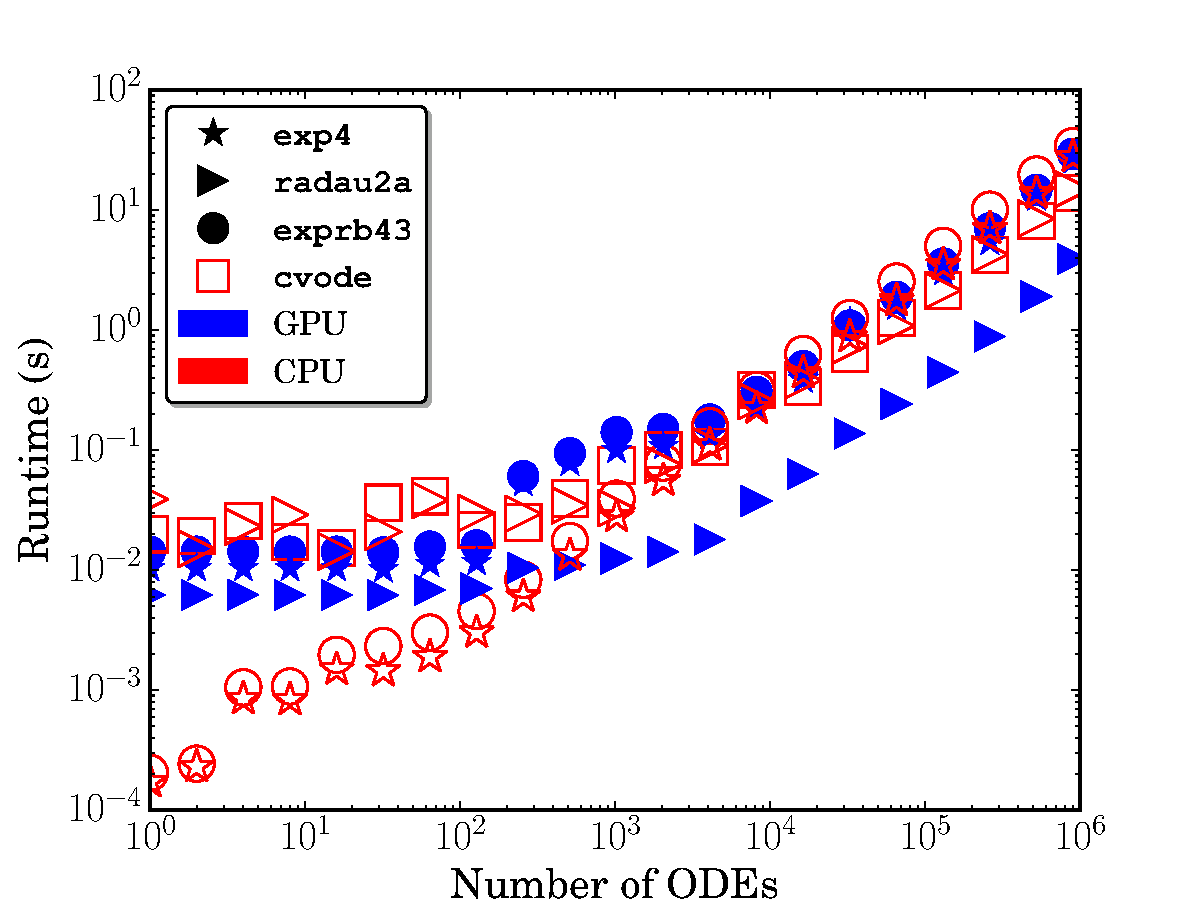
\includegraphics[width=\linewidth]{H2_1e-06_cpuvsgpu.pdf}
      \caption{$\delta t = \SI{1e-6}{\sec}$}   
  \end{subfigure}
  %\hfill
  \begin{subfigure}{0.49\textwidth}
      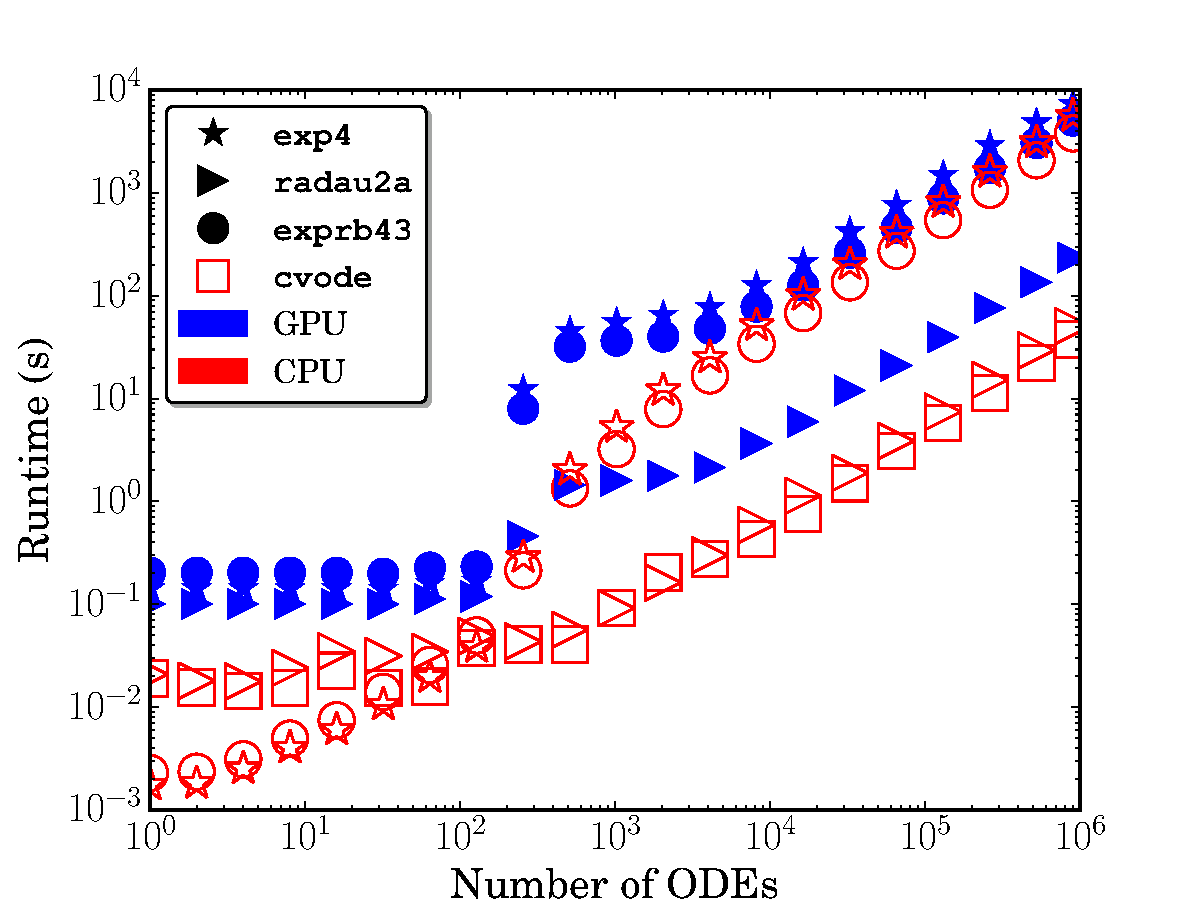
\includegraphics[width=\linewidth]{H2_1e-04_cpuvsgpu.pdf}
      \caption{$\delta t = \SI{1e-4}{\sec}$}
  \end{subfigure}
  \caption{Average runtimes of the integrators for the \ce{H2}\slash\ce{CO} model at two different global time-step sizes. 
  CPU versions ran in parallel on six cores.}
  \label{F:H2_perf}
\end{figure}

\begin{figure}[htb]
  \ifmeasure
  \fontsize{8pt}{10pt}\selectfont
  \fi
  \centering
  \begin{subfigure}{0.49\textwidth}
      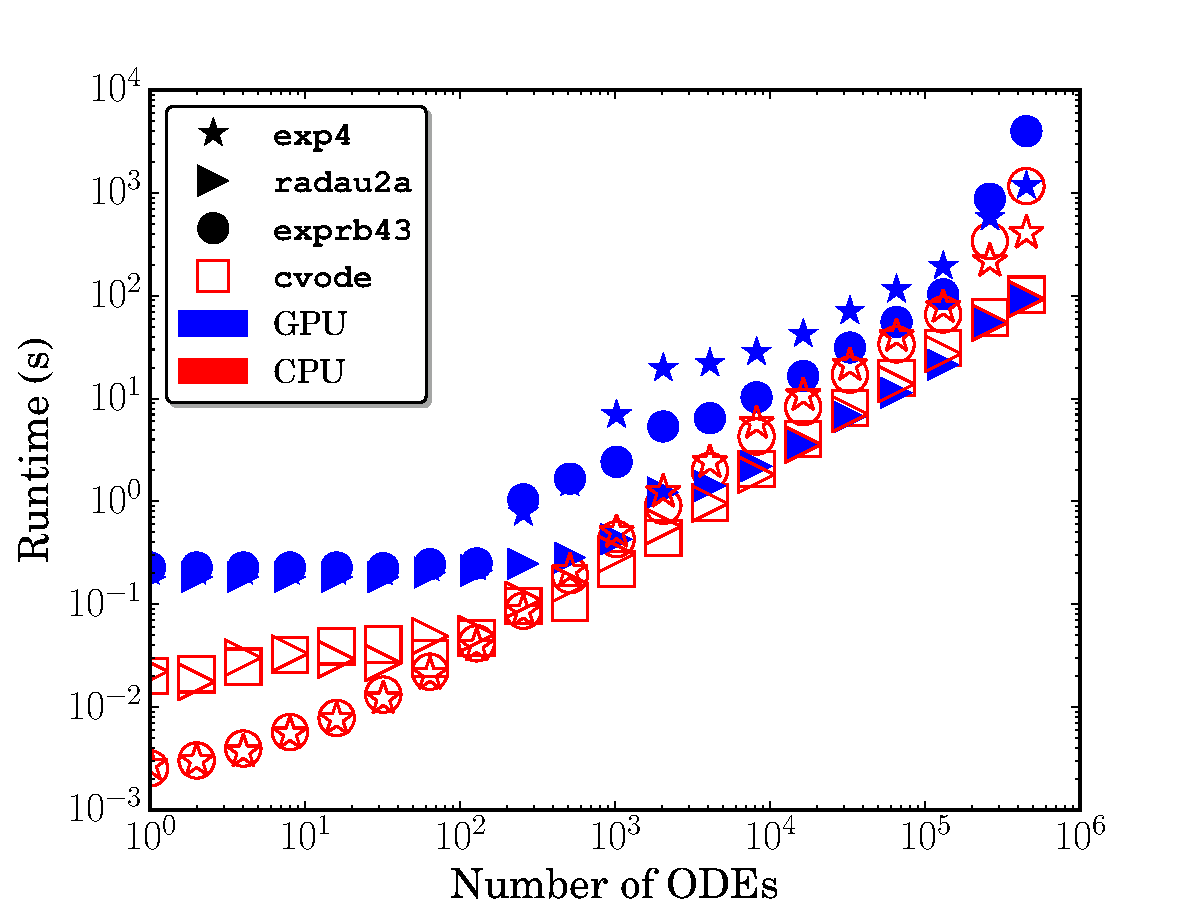
\includegraphics[width=\linewidth]{GRI_1e-06_cpuvsgpu.pdf}
      \caption{$\delta t = \SI{1e-6}{\sec}$}
  \end{subfigure}
  %\hfill
  \begin{subfigure}{0.49\textwidth}
      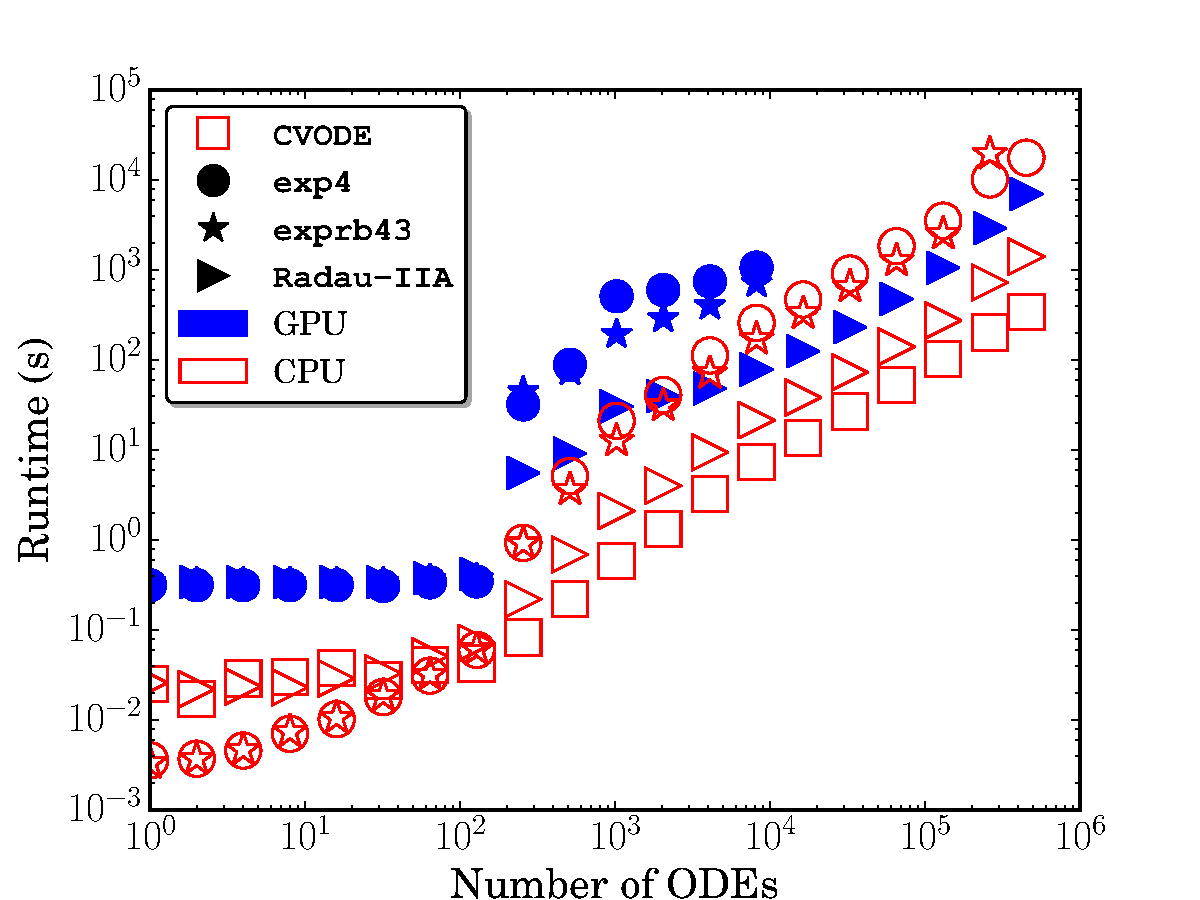
\includegraphics[width=\linewidth]{GRI_1e-04_cpuvsgpu.pdf}
      \caption{$\delta t = \SI{1e-4}{\sec}$}
  \end{subfigure}
  \caption{Average runtimes of the integrators for the GRI-Mech 3.0 model at two different global time steps. 
  CPU versions ran in parallel on six cores.
  Some of the longer-running exponential integration cases were omitted.}
  \label{F:GRI_perf}
\end{figure}

Figure~\ref{F:GRI_perf} shows the runtime of the integrators for the GRI-Mech 3.0 model.
The GPU \texttt{Radau-IIA} integrator outperformed \texttt{CVODE} for the smaller time-step size; at best, it ran \SI{31.5}{\percent} faster than \texttt{CVODE} (\num{131072} ODEs), and at worst was \SI{10}{\percent} faster (\num{16384} ODEs).
The larger time-step size again negatively impacted the performance of the GPU-based \texttt{Radau-IIA} integrator, dropping the performance to \num{8.63}$\times$ slower than \texttt{CVODE} at best (\num{32768} ODEs), and \num{20.48}$\times$ slower in the worst case (\num{450900} ODEs).
For the smaller time-step size the CPU \texttt{Radau-IIA} integrator was \SI{13}{\percent} faster than \texttt{CVODE} at best (\num{131072} ODEs) and \SI{10}{\percent} faster at worst (\num{450900} ODEs).
The larger time-step size---the stiffest case---was the only case where \texttt{CVODE} significantly outperformed CPU \texttt{Radau-IIA}, which was \num{2.66}$\times$ slower at best (\num{65536} ODEs) and \num{4.11}$\times$ slower at worst (\num{450900} ODEs).
This difference may be due to the adaptive-order nature of the \texttt{CVODE} algorithm, or potentially due to its maturity and years of optimization.
However, this effect is fairly minor and should not cause the order of magnitude decrease in relative performance between the GPU-based \texttt{Radau-IIA} integrator and \texttt{CVODE} observed when switching to the larger time step.

Two primary factors affect the performance of the GPU integration algorithms: chemical stiffness and thread divergence.
To investigate this further, we adopted a similar quantification of thread divergence to that of Niemeyer and Sung~\cite{Niemeyer:2014aa}:
\begin{equation}
	D = \frac{\sum_{i=1}^{32}{d_i}}{32 \max_{i \in 32} d_i} \;,
	\label{eqn:divergence}
\end{equation}
where $d_i$ is the number of internal integrator time steps taken to reach the global time step by thread $i$ in a warp (which consists of 32 threads).
$D$ represents the similarity of internal time step counts across threads in a warp---the most significant source of thread divergence.
If all threads in a warp use identical internal integration time steps and thus the warp experiences no thread divergence from this source, then $D = 1$; however, if a warp experiences an unbalanced number of internal integration time steps, then $D$ will tend to zero.

\begin{figure}[htb]
  \ifmeasure
  \fontsize{8pt}{10pt}\selectfont
  \fi
  \centering
  \begin{subfigure}{0.49\textwidth}
      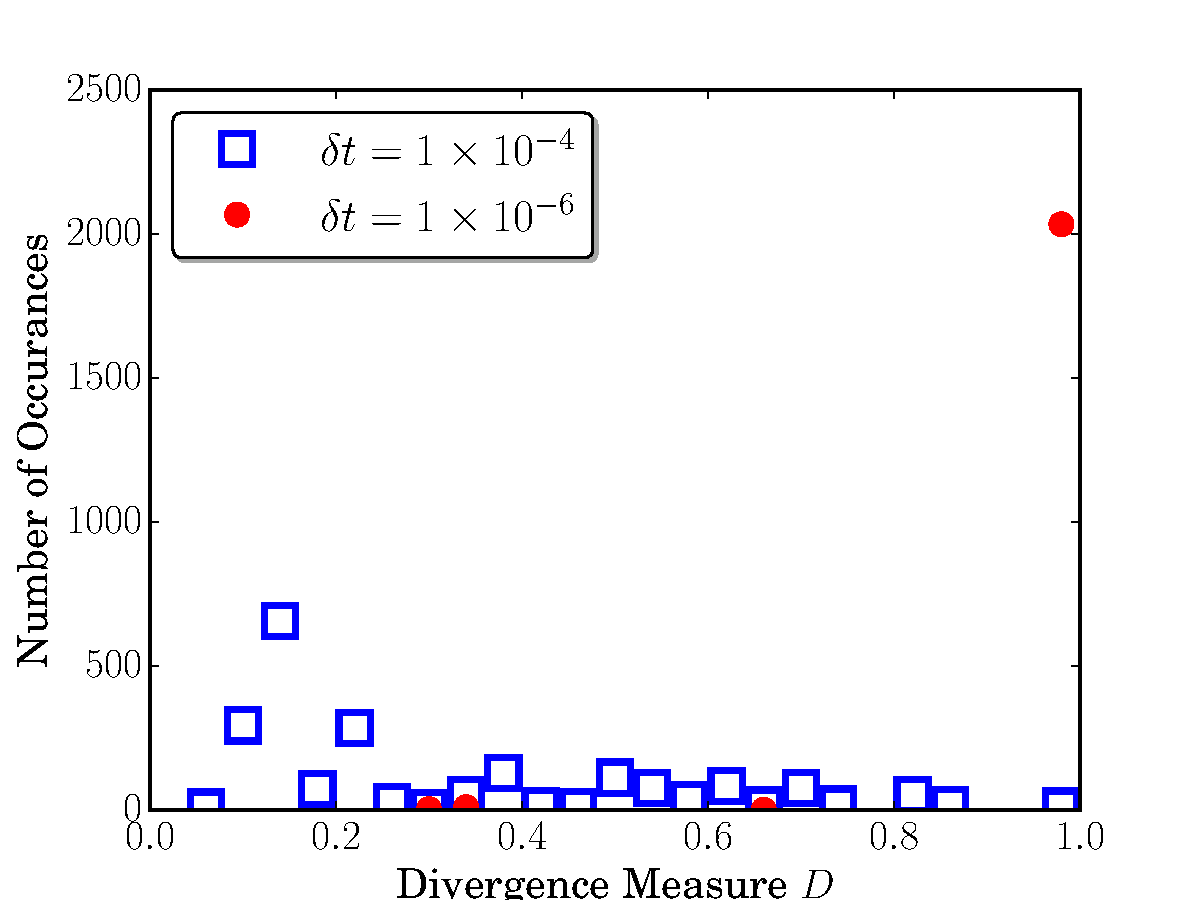
\includegraphics[width=\linewidth]{H2_radau2a_div.pdf}
      \caption{\ce{H2}\slash\ce{CO} model}
  \end{subfigure}
  %\hfill
  \begin{subfigure}{0.49\textwidth}
      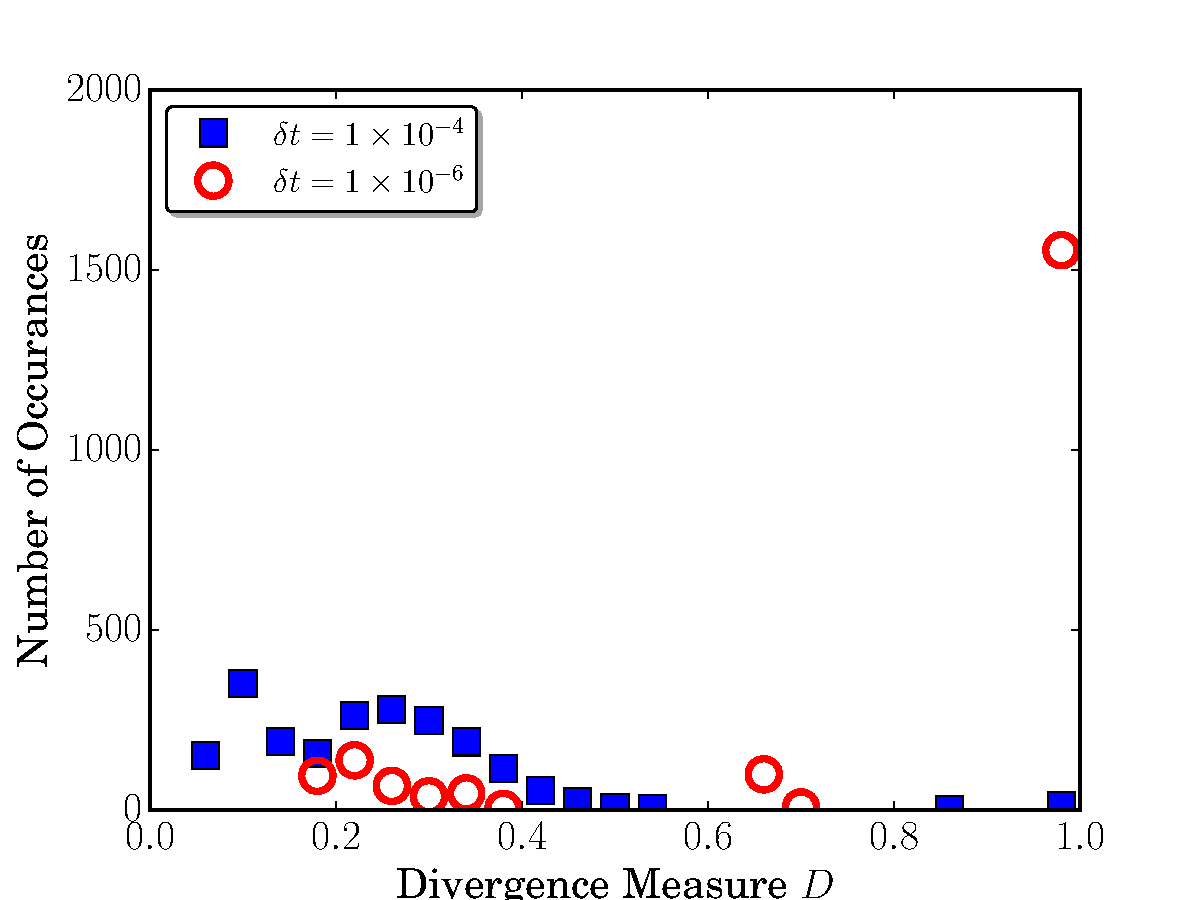
\includegraphics[width=\linewidth]{CH4_radau2a_div.pdf}
      \caption{GRI model}
  \end{subfigure}
  \caption{Thread divergence measure of the \texttt{Radau-IIA} solver for both models and time-step sizes.}
  \label{F:divergence}
\end{figure}

Figure~\ref{F:divergence} shows the distribution of the divergence measure $D$ for the \texttt{Radau-IIA} solver with both time-step sizes and kinetic models when run on \num{65536} ODEs, spread across \num{2048} warps.
For both kinetic models, increasing time-step size resulted in a sharp increase in the number of warps with large thread divergence (i.e., $D < 0.5$).
This implicates thread divergence, rather than chemical stiffness, as the main performance limiter for the GPU-based \texttt{Radau-IIA} integrator.
Furthermore, increased thread divergence likely caused the relative performance difference of the GPU \texttt{Radau-IIA} solver between the \ce{H2}\slash\ce{CO} and GRI-Mech 3.0 models at the smaller time-step size.
This observation motivates future work aimed at developing strategies to reduce thread divergence.
Potential solutions include adoption of an ODE per-block approach~\cite{Stone:2013aa}, reordering of ODEs to increase similarity of chemical stiffness inside a warp, or time-step synchronization between threads in a warp.

Figure~\ref{F:GRI_perf} also shows that the CPU exponential integrators are typically only \numrange{2}{3}$\times$ slower than \texttt{CVODE} for the smaller time-step size.
As the exponential integrators must only factorize a much smaller Hessenberg matrix (e.g., $5 \times 5$ for small integrator time-step sizes in stiff cases) rather than the entire Jacobian---as in the implicit integrators---significant savings in factorization can potentially be achieved with larger mechanism sizes.
For larger integrator time-step sizes without severe chemical stiffness (e.g., near equilibrium) the size of the Hessenberg matrix to be factorized typically grows to $20\times 20$.
However, as stiffness increases, e.g., as for the larger time-step size, the stability characteristics of the implicit integrators make them more favorable.
We hypothesize that the exponential integrators may be more efficient than the implicit integrators for moderately stiff systems (e.g., with small time-step sizes, or low tolerances) with larger chemical mechanisms.
Prior work~\cite{Niemeyer:2014aa} showed that stabilized explicit integrators can provide significant speedups for moderately stiff systems.
Although not shown in Fig.~\ref{F:divergence}, the GPU exponential integrators experienced significant thread divergence in all cases, and thus would also likely benefit from the thread divergence reduction techniques discussed above.

\subsection{Effect of shared memory caching}
\label{S:smem}

The effectiveness of the shared memory caching scheme was evaluated in several cases by comparing the mean runtime of the integrators using chemical source terms and analytical Jacobian subroutines generated with and without the caching algorithm enabled.
We observed typical speedups of $\SI{5}{\percent}$ and $\SI{10}{\percent}$ for the smaller and larger global time-step sizes, respectively.
This difference resulted from an increase in chemical source term and Jacobian evaluations required for the larger time-step size cases.
Even larger speedup factors were observed in certain cases with the GRI-Mech 3.0 model: a \SI{24.4}{\percent} speedup with \texttt{exp4} for \num{131072} ODEs and the \SI{e-6}{\second} time-step size, and a \SI{13.2}{\percent} speedup with \text{Radau-IIA} for \SI{32768} ODEs and the \SI{e-4}{\second} time-step size.
Thus, we recommend using this or a similar caching scheme in order to exploit shared memory in GPU integrators implemented on a per-thread basis.

\subsection{Limitations of per-thread local memory}

Through the course of this work, we encountered a significant but underdiscussed issue with the use of implicit and explicit exponential integrators on the GPU.
One goal of GPU-based chemical kinetic integration is to enable use of larger detailed mechanisms in realistic reacting flow simulations.
However, storage of the Jacobian on the GPU places severe restrictions on either the maximum allowable mechanism size or the total number of independent chemical-kinetic ODEs that can be solved concurrently.
For instance, the \texttt{Radau-IIA} solver requires storage of $N_s \times N_s$ matrices for the Jacobian, LU factorization, and complex LU factorization, where $N_s$ is the number of species in the mechanism.
Similarly, the exponential integrators require storage of matrices for the Jacobian, the Hessenberg and vector subspace resulting from the Arnoldi process, and the corresponding Hessenberg exponential.
While the Hessenberg, exponential Hessenberg , and vector subspaces may be smaller than the full Jacobian (e.g., by limiting the maximum Krylov subspace size), for the sake of simplicity in this analysis we assume full sizes.
This implies that storage requirements per ODE solved concurrently scale as $\mathcal{O}\left(3 \times N_s^2\right)$ for the \texttt{Radau-IIA} solver and as $\mathcal{O}\left(4 \times N_s^2\right)$ for the exponential solvers.

Per-thread local memory, which resides in device global memory, offers one option for storing these matrices and other integrator variables.
While this ensures coalesced memory access and simplifies indexing---both advantages from a programming standpoint---CUDA limits all threads to a maximum of \SI{512}{\kilo\byte} local memory, or \num{64000} double precision floating point numbers.
%This limits the maximum mechanism size to relatively small numbers, as Table~\ref{T:size_limits} shows, for GPU solvers implemented on a per-thread basis.
For example, even the USC Mech.~II model for \ce{C2H4}~\cite{Wang:2007} with 111 species caused the GPU to run out of local thread memory for our tests with all three GPU integrators.

Another option involves preallocating the Jacobian and associated matrices in global memory, and thus splitting the total global memory between all ODEs to be solved in a kernel launch.
This work used a Tesla C2075 GPU, similar to that used by recent GPU-based chemical kinetic integration studies~\cite{Shi:2011aa,Niemeyer:2011aa,Shi:2012aa,Le2013596,Stone:2013aa,Niemeyer:2014aa}---with \SI{6}{\giga\byte} of global memory and \num{e6} independent ODEs, this works out to just 750 doubles available per concurrent ODE.
Even assuming smaller problem sizes with \SI{e5} or \SI{e4} ODEs per kernel launch, each concurrent ODE is limited to just \num{7500} and \num{75000} doubles, respectively.
These limitations would severely constrain the allowable model sizes; for example, the \texttt{Radau-IIA} algorithm could handle models with approximately 15, 50, and 158 species for \num{e6}, \num{e5}, and \num{e4} concurrent ODEs, respectively.
%The resulting (approximate) maximum mechanism sizes are listed in Table~\ref{T:size_limits}.
%It is noted that this analysis applies equally to GPU solvers implemented both on a per-thread and per-block basis.
Sewerin and Rigopoulos~\cite{Sewerin20151375} discussed one approach to alleviate this issue: limiting the number of ODEs solved per kernel launch.
However, for larger models, e.g., \SIrange{250}{500} species, this issue may negatively impact performance by forcing kernel launches small enough to underutilize the GPU resources.
Otherwise, mechanism reduction (a priori or dynamic) may be employed to get around this complication.

%As one goal of GPU based integration algorithms is to enable use of larger, say \SIrange{100}{200} species, skeletal mechanisms in general reacting flow simulations through acceleration of chemical kinetic integration, the restrictive mechanism size\slash ODEs per kernel launch limits pose an issue.
%Thus we recommend use of global memory rather than per-thread local memory to store these matrices.
%In addition, a chemical kinetic Jacobian based on species concentrations instead of species mass fractions exhibits significantly greater sparsity~\cite{Lu:2009gh}, and thus may relax the mechanism size limits imposed by Jacobian storage.
%This increased sparsity will also result in acceleration of Jacobian evaluation and factorization, and other related linear algebra operations; this is an avenue that will be explored in future work.
%
%\begin{table}[htb]
%\centering
%\begin{tabular}{@{}l l l l@{}}
% \toprule
%& \multicolumn{3}{c}{Model Size Limit} \\
%Memory Type & \texttt{Radau-IIA} & \texttt{exp4} & \texttt{exprb43} \\
%\midrule
%Local	    & 146 & 126 & 126 \\
%
%Global (large)	    & 15 & 13 & 13 \\
%Global (reasonable) & 50 & 43 & 43 \\
%Global (low) & 158 & 136 & 136 \\
%\bottomrule
%\end{tabular}
%\caption{
%Approximate model species size limits for the various GPU integrators based on per-thread local memory and global memory limits.
%``Large'', ``reasonable'', and ``low'' refer to kernel launches with a total of \SI{e6}, \SI{e5} and \SI{e4} independent ODEs respectively
%}
%\label{T:size_limits}
%\end{table}

%%%%%%%%%%%%%%%%%%%%%%%%%%%%%%%%%%%%%%%%%%%%
\section{Conclusions}
\ifmeasure
\addvspace{10pt}
\fi
%%%%%%%%%%%%%%%%%%%%%%%%%%%%%%%%%%%%%%%%%%%%

The large size and chemical stiffness of chemical kinetic models relevant to fuels for transportation and power generation traditionally requires the use of high-order implicit integrators for efficient solutions.
Past work showed orders-of-magnitude speedups for solution of nonstiff to moderately stiff chemical kinetic systems using explicit solvers on GPUs.
In contrast, work on stiff chemical kinetic integration with implicit GPU solvers has been limited to specialized cases, or failed to surpass current CPU-based techniques.

This work demonstrated the performance of GPU-based integration methods, including an implicit fifth-order Runge--Kutta algorithm and two fourth-order exponential integration algorithms, using chemical source term and analytical Jacobian subroutines provided by the \texttt{pyJac} software~\cite{Niemeyer:2015im}.
For time-step sizes relevant to large eddy simulations, the GPU-based implicit Runge--Kutta method achieved a maximum speedup of over five compared with the CPU-based implicit \texttt{CVODE} integrator on a six-core CPU for an \ce{H2}\slash\ce{CO} model, and outperformed \texttt{CVODE} for the GRI-Mech 3.0 model by up to \SI{31.5}{\percent}; the exponential integrators performed worse in all cases.
For longer time-step sizes, the performance of all GPU solvers decreased significantly due to increased levels of thread divergence.
Furthermore, a shared memory caching algorithm was developed for the evaluation of chemical source terms and the analytical chemical Jacobian and resulted in modest performance benefits of \SIrange{5}{24}{\percent} speedup.
In addition, an issue was identified with storage of the Jacobian and similar matrices in per-thread local memory.

When compared with the results of a similar integration technique by Sewerin and Rigopoulos~\cite{Sewerin20151375}, our results showed that using an analytical chemical Jacobian matrix greatly improves implicit integration speeds on the GPU.
Further improvements to the analytical Jacobian code, e.g., by use of a chemical kinetic system based on species concentrations rather than mass fractions, are likely to further increase performance of the developed algorithms.
However, this work showed clearly that thread divergence poses the largest challenge to high performance of GPU-based integration techniques on a per-thread basis.
Therefore, our future work will focus on developing methods to mitigate and eliminate these effects.
Finally, new integration techniques such as hybrid implicit\slash explicit solvers, and selection of appropriate solvers based on estimated chemical stiffness, will be investigated.


%%%%%%%%%%%%%%%%%%%%%%%%%%%%%%%%%%%%%%%%%%%%%%%%%%%%%%%%%%%%%%%%%%%%%%
\section*{Acknowledgments}
\ifmeasure
\addvspace{10pt}
\fi

This material is based upon work supported by the National Science Foundation under grants ACI-1534688 and ACI-1535065.

\ifmeasure
\footnotesize
\baselineskip 9pt
\setlength{\bibsep}{0pt plus 0.3ex}
\fi
\bibliography{refs}
\bibliographystyle{elsarticle-num}

\end{document}
